\chapter{Bibliographie}
\section{Systèmes hybrides}

Cette partie a pour but de présenter les systèmes dynamiques hybrides, leurs problématiques, les différentes classes de systèmes hybrides ainsi que les différents outils de modélisation.
Nous nous appuierons fortement sur le travail de thèse de \cite{Kur02}, et plus particulièrement les parties 1.1 à 1.3. Étant donné que l'étude détaillée est faite dans ce travail de thèse, seule les idées principales sont reprises dans ce chapitre.

\subsection{Problématique}
Les systèmes automatisés actuels, de part leur complexité ne peuvent plus être représentés uniquement par leur comportement continu ou leur comportement discret, de nombreux systèmes réels sont à dynamique continue, mais supervisés ou contrôlés par une dynamique discrète. La modélisation de ces systèmes nécessitent une nouvelle approche et de nouveaux outils, c'est pourquoi ces dernières années de nombreux travaux vont dans ce sens et tentent de proposer des outils de modélisation et d'analyse.

\subsection{Classe de système hybride}
La nature hybride d'un système peut être inhérente aux phénomènes physiques qui le régissent, ou bien provoquée par une supervision de ce système. Il existe donc différentes classes de système hybride parmi lesquelles : 
\begin{itemize}
	\item \emph{Commutation autonome} : Caractérise un système qui va changer de façon discontinue lorsque l'état atteint certains seuils, c'est le cas des systèmes à hysteresis, la table de billard en est un exemple concret.
	\item \emph{Commutation contrôlée} : Traduit un phénomène où le système change de façon discontinue et instantanée en réponse à une entrée de commande, par exemple un système de thermostat. 
\end{itemize}

\subsection{Automate hybride}
La modélisation des systèmes dynamiques hybrides est un problème toujours en étude à ce jour \cite{goebel_hybrid_2012}. Le but est de réussir à trouver des outils permettant la représentation des dynamiques discrètes et continues dans une même syntaxe. L'automate hybride \cite{henzinger_theory_2000} est aujourd'hui un outil permettant de répondre à ces besoins. En effet, dans le domaine discret on représente très souvent les systèmes par un automate, en associant aux états des dynamiques continues, et en permettant aux transitions de dépendre elles aussi des conditions continues, il est possible de modéliser un système dynamique hybride.

\begin{figure}[h]
	\centering	
	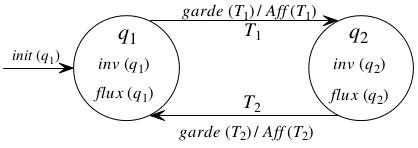
\includegraphics{images/automateHybride.jpeg}
	\caption{Automate hybride}
	\label{exempleAutomateHybride}
\end{figure}

L'\textit{état continu} du système est modélisé par un vecteur d'état continu $x(.)$ représentant un point dans un espace $X \subset \mathbb{R}^n$. Dans chaque sommet, la dynamique continue est modélisée par des conditions de flux telle que des équations différentielles ou des espaces d'états.

A chaque transition on associe un prédicat qui concerne l'état interne du système appelé \textit{garde}. Ce prédicat détermine les dates possibles pour le franchissement de la transition. Ainsi, une transition de l'automate hybride peut être franchie à l'instant $t$ si et seulement si sa garde est vérifiée par la valeur des variables d'état continues du système à l'instant considéré.

En général la garde d'une transition est exprimée par une région de l'espace d'état continu, qui peut se ramener à des intervalles.

L'ensemble des variables d'état continues mises à jour lors du franchissement d'une transition est décrit par une affectation. Les initialisations spécifiées par l'affectation correspondent à des fonctions, calculant la nouvelle valeur de l'état à partir de sa valeur avant le franchissement.

\begin{definition}{Un automate hybride d'ordre n, tel que présenté sur la figure \ref{exempleAutomateHybride} est défini par :}\\
\[\mathbb{A} = (Q, X, flux, inv, garde, Aff, init)\]
tel que :
\label{def:autom-hybride}
\begin{itemize}
\item Q = {$q_1, q_2, \ldots, q_m$} est un ensemble fini des sommets du graphe représentant les états discrets du système modélisé;
\item $X \subset \mathbb{R}^n$ est l'espace d'état continu. L'état continu du système est caractérisé à tout instant par le vecteur x = $[x_1, x_2, \ldots, x_n]^T$ dans l'espace Euclidien $\mathbb{R}^n$;
\item $flux(q_i)$ est la fonction qui affecte à chaque sommet une représentation pour l'évolution continue. Durant le séjour dans un sommet $q_i$ de l'automate hybride, l'évolution des variables continues est exprimée généralement sous la forme d'une équation d'état flux($q_i$) : $\dot{x} = \phi (q_i)(t,x,u)$, où $x \in X \subset \mathbb{R}^n$, $u \in U \subset \mathbb{R}^p$ et $\phi : X \times U \rightarrow X$;
\item L'invariant $inv(q_i)$ est une fonction qui associe à chaque sommet $q_i \in Q$ une contrainte sur les variables d'état continues x(.). Le système peut séjourner dans un sommet tant que l'invariant du sommet est satisfait;
\item $garde(T_i)$ est une fonction qui associe une condition de franchissement à chaque transition $T_i \in E$. Cette condition est en général une fonction logique entre des prédicats, portant sur les variables $x \in X$ et/ou ses dérivées $\dot{x} \in X$. Une transition $T_i \in E$ ne peut être franchie que si la condition $garde(T_i)$ est vraie;
\item L'affectation $Aff(T_i)$ est une fonction qui associe à chaque transition $T_i \in E$ une relation qui permet de mettre à jour la valeur des variables d'état après l'exécution de la transition $T_i$.
\item $init$ est une fonction qui affecte un état initial $x_0 \in X$ au sommet initial $q_{in} \in Q$. La condition initiale $init(q_{in})$ est un prédicat sur X.
\end{itemize}

\end{definition}

\section{Éléments de stabilité}
\subsection*{Introduction}
Le but de cette partie est d'apporter des éléments généraux mais nécessaires à la compréhension et à la réussite de mon travail de stage. Dans un premier temps quelques rappels seront effectués sur la modélisation d'un système linéaire par espace d'état, puis sur les notions d'équilibre et de stabilité de ces systèmes. Ensuite nous introduirons les notions de stabilité au sens de Lyapunov. Enfin nous ferons un point sur les inéquations linéaires matricielles (LMI en anglais), qui nous seront utiles pour Lyapunov. %Nous finirons par les outils d'analyse à notre disposition.

\subsection{Systèmes Linéaires}

\begin{definition} Modèle d'état\\
	\label{defmodeleEtat}
	Soit un système vérifiant les hypothèses de linéarité, sa représentation d'état est donnée par : 
	\[\dot{X}(t) = A(t).X(t) + B(t).U(t)\]
	\[Y(t) = C(t).X(t) + D(t).U(t)\]
	$X(t) \in \mathbb{R}^{n}$ est le vecteur d'état;\\
	$Y(t) \in \mathbb{R}^{r}$ est le vecteur de sortie;\\
	$U(t) \in \mathbb{R}^{m}$ est le vecteur des entrées;\\
	$A(t) \in \mathbb{R}^{n\times n}$ est la matrice dynamique;\\
	$B(t) \in \mathbb{R}^{n\times m}$ est la matrice de commande;\\
	$C(t) \in \mathbb{R}^{r\times n}$ est la matrice de mesure ou de sortie;\\
	$D(t) \in \mathbb{R}^{r\times m}$ est la matrice de transmission directe,
\end{definition}
Dans le cas général, un tel système est appelé système Linéaire à Temps Variant (LTV). Dans les cas particuliers où A, B, C et D sont constantes, le système est dit Linéaire à Temps Invariant (LTI).
Dans la suite nous considérerons les systèmes LTI.

\subsubsection{Notions de stabilité}
Parler de la stabilité d'un système est un abus de langage, en réalité nous devons parler de la stabilité d'un point d'équilibre, de fonctionnement ou d'une trajectoire de ce système.

\begin{definition} État d'équilibre\\
	\label{defEtatEq}
	Un point $X_e$ de la trajectoire d'état est un état d'équilibre (point d'équilibre) si $X(t_0) = X_e \Leftrightarrow X(t) = X_e, \forall t \geq t_0$ en l'absence de commande et de perturbations.\\
	Pour une représentation d'état comme vu précédemment, les points d'équilibre sont les solutions de l'équation : 
	\[\dot{X}(t) = 0_{n,1} \Leftrightarrow A.X(t) = 0_{n,1}\]
\end{definition}


\begin{theo}
	\label{theoAinversible}
	Un système continu LTI d'équations $\dot{X}(t) = A.X(t)$ peut avoir\\
	- Un point d'équilibre unique X = 0 si A est inversible\\
	- Une infinité de points d'équilibre si A n'est pas inversible	
\end{theo}

La stabilité permet de caractériser les points d'équilibre du système, c'est à dire que, si à un instant $t_0$, l'état d'équilibre est perturbé, l'état reviendra-t-il à cet état d'équilibre (stabilité) ou divergera-t-il (instabilité) ? Les différents types de stabilité sont présentés ci-après.

\begin{definition} Stabilité interne\\
	\label{defInterne}
	L'état d'équilibre $X_e$ est dit \textbf{stable} si
	\[ \forall \epsilon > 0, \exists\alpha > 0 \emph{ tel que si } ||X(0) - X_e|| \leq \alpha \emph{ alors } ||X(t) - X_e|| \leq \epsilon \forall t > 0\]	
	Dans le cas contraire, $X_e$ est dit \textbf{instable}.
\end{definition}

\begin{definition} Stabilité asymptotique\\
	\label{defAsymp}
	L'état d'équilibre $X_e$ est dit \textbf{asymptotiquement stable} si
	\[ \exists\alpha > 0 \emph{ tel que si } ||X(0) - X_e|| \leq \alpha \emph{ alors } \lim\limits_{t \rightarrow +\infty} X(t) = X_e \]
\end{definition}

\begin{definition} Stabilité exponentielle\\
	\label{defExpo}
	L'état d'équilibre $X_e$ est dit \textbf{exponentiellement stable} s'il existe $\alpha > 0$ et $\lambda > 0$ tels que 
	\[ \forall t > 0, \exists B_r(X_e,r), \forall X_0 \in B_r, ||X(t) - X_e|| \leq \alpha||X(0) - X_e||e^{-\lambda t} \]
	où $B_r(X_e,r)$ est une boule fermée de $\mathbb{R}^n$ de rayon $r$ et de centre $X_e$.
\end{definition}

\begin{rem}
	\label{remImplique}
	Il est possible de montrer que :
	\begin{center}
		stabilité exponentielle $\Rightarrow$ stabilité asymptotique $\Rightarrow$ stabilité interne
	\end{center}
\end{rem}

Pour finir sur les notions de stabilité d'un système LTI, nous allons regarder la caractérisation de la stabilité. Soit le point d'équilibre $X_e$ du système décrit par un modèle d'état comme présenté à la définition \ref{defmodeleEtat}, alors la caractérisation de la stabilité s'étudie à partir de la matrice A. A possède $n$ valeurs propres distinctes $\lambda_1,\ldots,\lambda_n$. Et nous avons le théorème suivant : 
\begin{theo} Conditions sur les valeurs propres (On note $R_e$ la partie réelle)\\
	$Re(\lambda_i) > 0$ si il existe $i \in 1,\ldots,n$, alors $X_e$ est \textbf{instable}\\
	$Re(\lambda_i) \leq 0$ pour tout $i \in 1,\ldots,n$, alors :\\
	\vspace{-1cm}
	\begin{tabbing}
		\hspace{1cm}\=\kill
		\> $Re(\lambda_i) < 0$ pour tout $i \in 1,\ldots,n$, alors $X_e$ est \textbf{asymptotiquement stable};\\ 
		\> $Re(\lambda_i) = 0$ et A diagonalisable, alors $X_e$ est \textbf{stable marginalement};\\ 
		\> $Re(\lambda_i) = 0$ et A non-diagonalisable, alors $X_e$ est \textbf{instable}.
	\end{tabbing} 
\end{theo}

\subsubsection{Méthode directe de Lyapunov pour l'étude de stabilité}
Considérons la stabilité du point d'équilibre 0 pour les systèmes étudiés, en effet d'un point de vue physique, la méthode de Lyapunov s'apparente à regarder l'évolution de la fonction d'énergie. Donc étudier le point d'équilibre 0 est équivalent à étudier à quel moment le système n'aura plus d'énergie. 

Pour tout point d'équilibre $x_e \neq 0$, on pose le changement de variable $\hat{x}(t) = x(t)-x_e$ et l'étude de la stabilité est identique à celle pour $x_e = 0$.
\begin{definition} Fonction candidate de Lyapunov\\
	\label{defFctLyap}
	Soit $V : \mathbb{R}^n \rightarrow \mathbb{R}_+$ une fonction telle que : 
	\begin{itemize}
		\item[i)] V est continûment différentiable en tous ces arguments
		\item[ii)] V est définie positive
		\item[iii)] Il existe a et b deux fonctions de $\mathbb{R}_+$ dans $\mathbb{R}_+$, continues, monotones, non décroissantes, telles que
		\[a(0) = b(0) = 0\]
		\[\forall x \in \mathbb{R}^n a(||x||) \leq V(x) \leq b(||x||)\]
		alors V est une fonction candidate de Lyapunov.
	\end{itemize}
\end{definition}

\begin{rem}
	La définition implique que la fonction V définit des équipotentielles imbriquées. C'est à dire que les courbes V(x) = cste, appelées \textbf{équipotentielles de Lyapunov}, définissent des domaines convexes autour de l'origine.
\end{rem}

\begin{theo} Stabilité locale\\
	Si il existe une fonction $V$ dont les dérivées partielles premières sont continues et telle que :
	\begin{itemize}
		\item[1-] V est une fonction candidate de Lyapunov (Cf. définition \ref{defFctLyap})
		\item[2-] $\dot{V}$ est localement semi-définie négative dans un voisinage de l'origine $\Omega$.
	\end{itemize}
	
	Alors le point d'équilibre 0 est \textbf{stable} et un domaine de conditions initiales stables est délimité par n'importe quelle équipotentielle de Lyapunov contenue dans $\Omega$.\\
	Si $\dot{V}$ est localement définie négative dans $\Omega$, alors la stabilité est dite \textbf{localement asymptotique} dans la partie de l'espace délimitée par n'importe quelle équipotentielle de Lyapunov contenue dans $\Omega$.
\end{theo}

\begin{theo} Stabilité globale asymptotique\\
	\label{theoStabLyap}
	S'il existe une fonction V telle que
	\begin{itemize}
		\item[1-] V est une fonction candidate de Lyapunov
		\item[2-] $\dot{V}$ est définie négative
		\item[3-] La condition $||x|| \rightarrow +\infty$ implique $V(x) \rightarrow +\infty$
	\end{itemize}
	alors 0 est un point d'équilibre globalement asymptotiquement stable.
\end{theo}

Le problème de cette méthode de Lyapunov est de trouver une fonction de Lyapunov pour le système considéré, en effet dans le cas non-linéaire il n'existe pas de méthode systématique. Dans le cas des systèmes LTI, il existe forcément une fonction de Lyapunov, mais elle n'est pas évidente à trouver.

\subsubsection{Application aux systèmes linéaires}
Dans ce cas, la représentation du système est donc classique : $\dot{x} = Ax$. Le point d'équilibre candidat est nécessairement $x = 0$. En choisissant $V(x) = x^TPx$ avec $P$ symétrique et définie positive ($P = P^T > 0$), la condition de stabilité asymptotique (Cf. Théorème \ref{theoStabLyap}) s'écrit alors 
\begin{center}
	$   \left \{
	\begin{array}{c c l}
	V(x) = x^TPx & > & 0, \forall x \\
	\dot{V}(x) = x^T(A^TP + PA)x & < & 0, \forall x
	\end{array}
	\right. $
\end{center}

\begin{theo}
	Le système $\dot{x} = Ax$ est stable si et seulement si il existe une matrice définie positive P vérifiant le système LMI suivant : 
	\begin{center}
		$   \left \{
		\begin{array}{r c l}
		P & > & 0 \\
		A^TP + PA & < & 0
		\end{array}
		\right. $
	\end{center}
\end{theo}

\begin{theo}
	Dans le cas d'un système discret du type $x_{k+1} = Ax_k$, le théorème de stabilité devient (Lemme de Schur) :
	\begin{center}
		$   \left \{
		\begin{array}{r c l}
		P & > & 0 \\
		A^TPA - P & < & 0
		\end{array}
		\right. $
	\end{center}
	\label{theo:lyapDiscret}
\end{theo}
%\pagebreak
%Par la suite nous travaillerons avec des systèmes LTI discret soumis à une commande, d'après les travaux de \cite{zhai_analysis_2007}, les conditions LMI deviennent : 
%\begin{theo}
%	Dans le cas d'un système discret du type $   \left \{
%	\begin{array}{l}
%	x_{k+1} = Ax_k + Bu_k \\
%	y_k = Cx_k + Du_k
%	\end{array}
%	\right. $ :
%	\begin{center}		
%		$   \left \{
%		\begin{array}{c c l}
%		P & > & 0 \\
%		\begin{bmatrix}
%		A^TPA-P+C^TC	& A^TPB + C^TD \\ 
%		B^TPA + D^TC	& B^TPB - I + D^TD  
%		\end{bmatrix} & < & 0
%		\end{array}
%		\right. $
%	\end{center}
%	\label{theo:lyapDiscretAvecEntree}
%\end{theo}
%
%De plus, dans le cas où nous ne souhaitons pas considérer les sorties du système, le théorème précédent devient :
%\begin{center}		
%	$   \left \{
%	\begin{array}{c c l}
%	P & > & 0 \\
%	\begin{bmatrix}
%	A^TPA-P	& A^TPB \\ 
%	B^TPA	& B^TPB - I  
%	\end{bmatrix} & < & 0
%	\end{array}
%	\right. $
%\end{center}
%\label{theo:lyapDiscretAvecEntree}

\pagebreak
\subsubsection{Application aux systèmes hybrides}
\label{subsubsec:applicationStabHybride}
Par la suite nous allons travailler avec des systèmes hybrides. Chaque état de notre système hybride est un modèle d'état linéaire discret, de plus nous souhaitons pouvoir prendre en compte les entrées de notre système dans l'étude de la stabilité.

Dans \cite{mignone_stability_2000} est présenté une approche d'étude de la stabilité des systèmes hybride utilisant les approches LMI et Lyapunov présenté ci-dessus. Le but de cette approche est de pouvoir garantir la stabilité locale (donc la décroissance de la fonction d'énergie au sein d'un état), mais aussi une décroissance globale, garantissant que les changements de modes de vont pas venir déstabiliser le système.

Le théorème \ref{theo:lyapDiscret} devient donc : 
\begin{theo}
	Dans le cas d'un système discret du type $x_{k+1} = Ax_k$ :
	\begin{center}
		$   \left \{
		\begin{array}{r c l l}
		P_i & > & 0 & \forall i\\
		A_j^TP_iA_j - P_j & < & 0 & \forall (j,i)
		\end{array}
		\right. $
	\end{center}
	\label{theo:lyapDiscretHybride}
\end{theo}

Une extension de ce théorème est également présenté dans cet article pour la prise en compte des entrées du système.

\label{subsubsec:stabHybride}
Dans le cadre de ce stage l'étude de la stabilité doit être appliquée à des systèmes hybrides. Des analyses s'appuyant sur la théorie de Lyapunov décrite précédemment sont développés dans \cite{shorten_stability_2007}\cite{oehlerking_decomposition_2011}.

Le principe est de trouver une fonction d'énergie $V_i$ par mode telles que pour tout mode $m_i \in M$ et pour tout $x$ : 
\[ \frac{\delta V_i}{\delta x} \times f(x,m_i) < 0\]
De plus, lors des commutations entre les modes $i$ et $j$, on doit s'assurer que globalement, l'énergie du système (donc la fonction $V$) diminue : 
\[ V_j(x)-V_i(x) \leq 0 \]

\noindent
\shadowbox{\begin{minipage}{\textwidth}
		\textbf{Résumé pour l'étude de la stabilité : }
		\begin{itemize}
			\item[1-] Trouver les points d'équilibre du système en résolvant Ax = 0
			\item[2-] Linéariser le système autour des points d'équilibre pour évaluer la stabilité/instabilité des points d'équilibre (cette étape est souvent appelée première méthode de Lyapunov). Au voisinage d'un point d'équilibre $x_e$ :
			\[\dot{x} = f(x) = A(x-x_e) + o(x-x_e)\]
			Si la matrice A est définie négative, le système est localement asymptotiquement stable autour de $x_e$, mais aucun domaine de conditions initiales stables ne peut-être déterminé à ce stade.
			Si A est semi-définie négative, on ne peut pas conclure. Sinon le point d'équilibre est instable.
			\item[3-] Choisir une fonction candidate de Lyapunov V et, en posant le changement de variable \^{x} = x - $x_e$, étudier les domaines de stabilité/instabilité à l'aide de la seconde méthode de Lyapunov.
			\item[4-] Si les résultats ne sont pas concluants, choisir une autre fonction de Lyapunov et recommencer.
			\item[5-] Pour l'hybride : trouver une fonction de Lyapunov pour chaque mode et vérifier la décroissance globale de l'énergie du système. 
		\end{itemize} 
	\end{minipage}} 
%\subsubsection{Résumé pour l'étude de la stabilité}


%\subsubsection{Utilisation de MatLab pour l'étude de la stabilité (Lyapunov + LMI)}
%Cf. LyapunovLin.m pour un exemple de vérification de la seconde méthode de Lyapunov. Et voir switch\_test2.m pour avoir un exemple de projection des ellipses dans les différents plans de l'espace.
%
%\subsection{Éléments divers}
%Cette section va nous permettre de présenter différents points qui pourront être intéressants par la suite
%
%\subsubsection{D-stable}
%Une Matrice carré réelle A est dite (Hurwitz) D-stable si pour toute matrice diagonale positive D, la matrice DA est (Hurwitz) stable (à valeur propre strictement négative).
%
%Une matrice A est dites Hurwitz diagonalement stable si il existe une matrice positive P diagonale tel que A'P+PA est définie négative.
%
%A est Schur diagonalement stable si il existe une matrice positive P diagonale tel que A'PA-P est définie négative.
%
%Hurwitz diagonale stabilité est une condition suffisante pour la D-stabilité, mais l'inverse n'est vrai que pour une certaine classe de matrice. (Cf. On discrete-time diagonal and D-stability)


%\end{document}
\pagebreak
\section{Planification}
%\subsection*{Introduction}
La commande automatique d'un système discret peut se faire par la synthèse de plans. On présente ici le cadre classique de planification, puis des approches appliquées aux robots aériens, enfin des approches à base de contraintes qui semblent être les mieux adaptées à nos besoins.

%Un algorithme de planification peut être décrit comme un algorithme produisant un plan à partir des entrées suivantes :
%\begin{itemize}
%\item Une description du monde, de l'environnement;
%\item Une liste d'actions possibles;
%\item Un ensemble de buts à atteindre.
%\end{itemize}
%Un plan est défini comme un ensemble d'actions et de contraintes entre ces actions. Ces contraintes permettent d'ordonner les actions entre elles pour assurer l'exécution du plan.
\subsection{Modèle de description}

La première étape pour un algorithme de planification est de définir les données d'entrée sur lequel il agira : c'est le modèle de description qu'il utilisera pour représenter le monde.

Plusieurs paradigmes ont été proposés depuis les premiers travaux sur la planification. Ces paradigmes se distinguent en fonction de plusieurs critères :

\begin{itemize}
	\item La facilité d'utilisation : par exemple la quantité de travail nécessaire pour en comprendre ou écrire un problème;
	\item La puissance de représentation : tous les langages ne permettent pas de représenter les mêmes contraintes;
	\item La qualité de l'écosystème : le nombre de planificateurs utilisant le même type de modèle ou de problème ainsi que les outils disponibles.
\end{itemize}

Dans cette partie nous présenterons la planification d'un point de vue générale, ensuite nous parlerons de deux formalismes de planification (STRIPS et PDDL), par la suite nous présenterons quelques approches d'architectures de planification pour des missions de drone, et nous finirons par la présentation du formalisme des CSP afin de les appliquer sur des problèmes de planification. 

\subsubsection{Description par état}

La représentation sans doute la plus simple pour la planification est une représentation du monde sous forme d'un graphe. Chaque état possible du monde est alors un nœud, et chaque arête représente une action qui fait passer d'un état à un autre.

\begin{definition}Planification en tant que recherche dans un graphe\\
	\label{def:plannif_etat}Un problème de planification est défini par :
	\begin{itemize}
		\item $S$ un ensemble d'état;
		\item $A$ un ensemble d'action;
		\item $f : S \times A \to S$ une fonction partielle;
		\item $I \in S$ l'état initial;
		\item $S_G \subset S$ : un ensemble d'état but.
	\end{itemize}
\end{definition}

La fonction $f$ permet de calculer l'état suivant étant donné l'état courant et l'action appliquée.
Elle permet donc de définir un graphe orienté dont les nœuds sont $S$.

Le problème de planification revient alors à chercher un chemin dans ce graphe depuis $I$ vers n'importe quel nœud de $S_G$.

Bien que simple théoriquement, l'explosion combinatoire du nombre d'états rend ce modèle inadapté à une utilisation concrète. En effet le nombre d'état à représenter augmente exponentiellement avec le nombre d'objet dans le problème.
%\pagebreak
\subsubsection{STRIPS}

Pour palier à ce problème d'explosion combinatoire du nombre d'états, le formalisme STRIPS \cite{STRIPS} utilise une représentation factorisée des états. Ce formalisme a été introduit par le premier planificateur robotique, appelé STRIPS, développé pour le robot Shakey \cite{Shakey}.

L'idée est de ne pas représenter chaque état comme une seule entité mais de le séparer en différentes composantes : la position de chaque robot par exemple. Un état est alors défini comme un ensemble de fluents prenant la valeur vrai ou faux. Chaque fluent peut être vu comme une propriété qui est vérifiée ou non dans un état donné : par exemple "le robot $r_1$ est au point $pt_1$" ou "l'acquisition $a_1$ a été réalisée".

\begin{definition}Problème de planification (STRIPS)\\
	\label{def:prb_strips}Un problème de planification est défini par :
	\begin{itemize}
		\item Un ensemble $F$ de fluents
		\item Un ensemble d'action $A$
		\item Un ensemble $I \subseteq F$ représentant l'état initial
		\item Un ensemble $G \subseteq F$ représentant le but
	\end{itemize}
\end{definition}

\begin{definition}Etat (représentation STRIPS)\\
	\label{def:etat_strips}
	Etant donné un problème de planification $\left<F,A,I,G\right>$, un état est défini comme sous-ensemble de $F$.
\end{definition}

\begin{definition}Action (représentation STRIPS)\\
	\label{def:action_strips}Soit $F$ un ensemble de fluents, une action est définie par
	\begin{itemize}
		\item Un nom unique dans le problème considéré
		\item Un ensemble $Pre \subseteq F$ de pré-condition
		\item Un ensemble $Eff \subseteq F$ de d'effet
		\item Un ensemble $Del \subseteq F$ d'effacement
	\end{itemize}
\end{definition}

L'application d'une action $a = \left<Pre, Eff, Del\right>$ n'est applicable à un état $e$ si et seulement si $e \subseteq Pre$ et produit alors l'état $((e \cap \neg Del) \cup Eff)$. On note alors l'application d'une action dans un état $a[e] = ((e \cap \neg Del) \cup Eff)$.

L'objectif de la planification est alors de trouver une séquence d'actions tel quel chaque action soit applicable (c'est à dire que ses pré-conditions sont vérifiées au moment de son exécution) et que l'état final contienne $G$. Formellement on peut définir un plan comme une séquence d'action :

\begin{definition}Plan (représentation STRIPS)\\
	\label{def:plan_strips}Étant donné un problème de planification $\left<F,A,I,G\right>$, un plan est défini comme une séquence d'actions $\left<a_0, a_1, ..., a_n \right>$ de $A$. 
\end{definition}

Un plan produit une séquence d'état $\left<e_0, e_1, ... e_n\right>$ définie par $e_0 = I$ et $\forall i > 0, e_{i+1} = a_i[e_i]$. 

\begin{definition}Plan solution (représentation STRIPS)\\
	\label{def:solution_strips}Un plan est valide si et seulement si $\forall i, Pre(a_i) \subseteq e_i$.\\	
	Un plan est solution du problème $\left<F,A,I,G\right>$ si et seulement si il est valide et $G \subseteq e_n$.
\end{definition}

On définit de plus l'\emph{horizon} d'un problème de planification comme la limite supérieure de la longueur des plans considérés.

L'intérêt de cette représentation est de permettre une description beaucoup plus compacte des actions : au lieu de devoir décrire toutes les transitions possibles on décrit l'effet d'une action sur l'ensemble des états possibles à la fois. De ce point de vue, STRIPS représente une très nette amélioration en terme de praticité d'utilisation vis à vis de la description par un graphe. Par contre la puissance de représentation est la même.

\subsubsection{PDDL}

PDDL \cite{pddl1998} est une évolution du formalisme STRIPS couramment utilisée pour les compétitions internationales de planification \footnote{\url{http://icaps-conference.org/index.php/Main/Competitions}} des conférences ICAPS.
PDDL utilise des variables dans la description des actions ce qui permet une description compacte des problèmes.
Les problèmes sont aussi divisés en deux parties, le \emph{domaine} et le \emph{problème}.
Le \emph{domaine} contient des informations générales sur les actions disponibles et leurs effets en utilisant une description principalement sous forme de variables.
Le \emph{problème} au sens PDDL rassemble les informations sur les objets présents (permettant l'instanciation des variables du domaine), l'état initial et le but à atteindre.

Ce langage étant assez répandu grâce aux compétitions des IPC, son écosystème est assez riche. 
Tous les planificateurs concourants aux IPC sont disponibles, ainsi que les problèmes utilisés.
De plus, un vérificateur de plan, permettant de tester la validité d'un plan sur un domaine et un problème donné, est également disponible.

Plusieurs évolutions ont été proposées à PDDL : une représentation des problèmes temporels et de variables numériques \cite{Fox2003}, les prédicats dérivés et les conditions initiales temporelles \cite{Edelkamp2004}.% des aspect multi-agent \cite{Kovacs2011} ou encore les métriques à utiliser \cite{Gerevini2006}.

\subsubsection*{Représentation du temps dans PDDL}
\label{sec:pddl_time}

Une des limitations de toutes les représentations présentées précédemment est leur puissance de représentation limitée : les plans ne sont qu'une succession linéaire d'actions sans notion temporelle. 
La version 2.1 \cite{Fox2003} propose une extension temporelle. 
Elle permet de doter les actions d'une durée et de faire référence aux dates de début et de fin de chaque action pour les pré-conditions et les effets.
Cela permet d'imposer des actions en parallèles ou au contraire en interdire le chevauchement.

La définition d'un problème et d'un état est reprise de la formulation STRIPS (respectivement la définition \ref{def:prb_strips} et \ref{def:etat_strips}).
Par contre les actions sont définies avec des contraintes temporelles.
Ces contraintes sont exprimées avec des \emph{étiquettes temporelles}.

%\begin{definition}Fluent temporel (PDDL2.1)\\
%	\label{def:fluent_temp_pddl21}
%	Soit $F$ un ensemble de fluents.\\
%	Un fluent temporel est défini comme une paire $\left< f, t \right>$ où $f \in F$ est un fluent et $t$ est une étiquette temporelle $t \in \left\lbrace overall, atstart, atend \right\rbrace $.\\
%	On note $\tilde{F}$ l'ensemble des fluents temporels.
%\end{definition}
%
%\begin{definition}Action (PDDL2.1)\\
%	\label{def:action_pddl21}
%	Soit $F$ un ensemble de fluents.\\ Une action est définie par :
%	\begin{itemize}
%		\item Un nom unique dans le problème considéré
%		\item Une durée $d \in \mathbb{R}$
%		\item Un ensemble $Pre \subseteq \tilde{F}$ de pré-condition
%		\item Un ensemble $Eff \subseteq \tilde{F}$ d'effets
%		\item Un ensemble $Del \subseteq \tilde{F}$ d'effacements.
%		
%		De plus, les étiquettes temporelles $overall$ ne peuvent être utilisées que pour les pré-conditions d'une action.
%	\end{itemize}
%\end{definition}
%
%Les conditions d'application d'une action et ses effets dépendent donc des étiquettes temporelles.
%Une action n'est applicable que si toutes ses pré-conditions sont valides.
%Une pré-condition $\left< f, t \right>$ est ainsi valide :
%\begin{itemize}
%	\item Si $t = atstart$ et que $f$ est vrai au début de l'action
%	\item Si $t = atend$ et que $f$ est vrai à la fin de l'action
%	\item Si $t = overall$ et que $f$ est vrai sans discontinuer du début à la fin de l'action (ces deux points étant exclus de l'intervalle)
%\end{itemize}
%Un effet se réalise soit au début de l'action (si $t = atstart$) soit à la fin de l'action (si $t = atend$).
%
%\begin{definition}Plan (PDDL2.1)\\
%	Soit $\left<F,A,I,G\right>$ un problème de planification.\\
%	Un plan est défini comme une séquence d'action datées : $\left< \left< t_0, a_0 \right>, ... \left< t_n, a_n \right> \right>$ où $\forall i, a_i \in A$ et $t_i \in \mathbb{R}$ représente la date de début de $a_i$.
%\end{definition}
%
%Pour tout action $a_i$ de durée $d_i$, si $t_i$ est sa date de début alors $t_i + d_i$ est sa date de fin. Pour simplifier les notations, on notera alors $t^i_i$ et $t^f_i$ respectivement sa date de début et sa date de fin. 
%
%Les actions d'un plan pouvant se chevaucher, il est nécessaire de raisonner sur l'enchaînement des dates de début et de fin des actions. 
%PDDL2.1 ne permet pas d'ajouter des contraintes ou de modifier l'état courant en dehors de ces points particuliers.
%On parle alors d'évènement pour désigner ses points particuliers, le premier étant l'instant initial du plan.
%
%\begin{definition}Évènement (PDDL 2.1)\\
%	Soit $\Pi = \left<F,A,I,G\right>$ un problème de planification. \\
%	Soit $p = \left< \left< t_0, a_0 \right>, ... \left< t_n, a_n \right> \right>$ un plan.\\
%	On note l'ensemble des \emph{événements} $E = \left< e_0, ... e_m\right>$ tel que $\forall i, t^i_i \in E, t^f_i \in E$, $e_0 = 0$ et $\forall i, e_i \leq e_i+1$.
%\end{definition}
%
%L'état courant après un évènement $e_i$, noté $s[e_i]$, est donc l'état précédent modifié par les effets de toutes les actions s'appliquant à ce moment là (les effets et effacement étiquetés $atend$ est actions finissant en $e_i$ ainsi que les effets et effacement étiquetés $atstart$ des actions commençant en $e_i$).
%De plus, $s[e_0] = I$.
%On note $precedent(e_{i+1}) = e_i$.
%
%\begin{definition}Plan valide (PDDL 2.1)\\
%	Soit $\Pi = \left<F,A,I,G\right>$ un problème de planification. \\
%	Soit $p = \left< \left< t_0, a_0 \right>, ... \left< t_n, a_n \right> \right>$ un plan.\\
%	Soit $E = \left< e_0, ... e_m\right>$ la liste ordonnées des évènements.\\
%	Un plan est valide si et seulement si toutes les pré-conditions de ses actions sont valides :
%	$\forall i, \forall \left< f, t \right> \in Pre(a_i) :$
%	\begin{itemize}
%		\item Si $t = atbegin$ : $f \in s[precedent(t^i_i)]$
%		\item Si $t = atend$ : $f \in s[precedent(t^f_i)]$
%		\item Si $t = overall$ : $\forall e, t^i_i \leq e < t^f_i, f \in s[e]$
%	\end{itemize} 
%\end{definition}
%
%De plus, si des actions venaient à produire et consommer un fluent au même instant ou à produire et détruire un même fluent, alors ces deux actions doivent être temporellement séparées pour lever les ambiguïtés.
%De plus amples détails sont disponibles dans la définition du langage \cite{Fox2003}.
%
%\begin{definition}Plan solution (PDDL 2.1)\\
%	Soit $\Pi = \left<F,A,I,G\right>$ un problème de planification. \\
%	Soit $p = \left< \left< t_0, a_0 \right>, ... \left< t_n, a_n \right> \right>$ un plan.\\
%	$p$ est solution de $\Pi$ ssi. $p$ est valide et $G \subset s[e_n]$. 
%\end{definition}

Le langage PDDL2.1 étant conçu comme une extension au PDDL, toutes les descriptions PDDL antérieurs sont des descriptions valides en PDDL2.1.

\begin{theo}Conversion de STRIPS vers PDDL2.1\\
	On peut montrer que toute solution à un problème STRIPS est solution d'un problème PDDL2.1 où toutes les pré-conditions reçoivent l'étiquette $overall$ et tous les effets reçoivent l'étiquette $atend$.
\end{theo}

\subsection{La planification appliquée aux mission de drone}
\cite{chanthery_planification_2005} présente une architecture très intéressante pour le problème de planification de mission pour un drone : 
\begin{itemize}
	\item niveau 3 : gestion de la mission et de son environnement, ce niveau permet de prendre en compte une modification de l'environnement de mission du drone, et donc de demander un nouveau plan (niveau 2)
	\item niveau 2 : Gestion du plan, ce niveau permet le calcul effectif d'un plan (demandé par le niveau 3, ou le niveau 1 si un segment du plan n'est pas conforme)
	\item niveau 1 : Gestion de la trajectoire, ce niveau permet le calcul d'une trajectoire pour le segment de plan donné par le niveau 2, il doit ressortir l'ensemble des points que doit suivre le drone pour réaliser ce segment du plan, si le niveau 0 considère que le prochain point n'est pas atteignable, le niveau 1 doit calculer une nouvelle trajectoire pour ce même segment
	\item 0 : guidage, ce niveau permet le guidage du drone, il doit informer le niveau 1 si le prochain point est atteignable ou pas, si il l'est, il demande à la couche de commande d'effectuer les actions nécessaires pour aller à ce point (modification de l'angle d'incidence, augmentation de la poussée etc...
\end{itemize}
Dans ce travail, les niveaux 3 et 2 ont été traités (avec une méthode basée sur un algorithme A*), les niveaux inférieurs ont été considérés comme connus. Le niveau 1 peut être vu comme du motion planning (un drone est vu comme un robot non-holonome), le niveau 0 lui peut être vu comme la boucle de commande du drone (modélisation continu, contraintes LMIs pour la stabilité), mais cette commande doit intégrer des aspects discret (mission) et continu (mécanique du vol, stabilité), nous pouvons donc émettre l'hypothèse qu'un modèle hybride pourrait permettre la modélisation de cet étage.

Dans le monde de la robotique il existe une sous branche du motion planning : Kinodynamic planning \cite{masoud_kinodynamic_2010}, c'est à dire que l'on va prendre en compte (dès la phase de planification) la dynamique du robot (contrainte non-holonome, stabilité ...)
Alors qu'avec l'architecture proposée dans \cite{chanthery_planification_2005}, le niveau 2 donne un plan non contraint par la dynamique, le niveau 1 donne une trajectoire elle aussi non contrainte par la dynamique, et c'est seulement le niveau 0 qui est capable de faire remonter des informations sur l'aspect réalisable du mouvement ou pas.

%\subsection{Thèse DICHEVA 2012}
\cite{dicheva_planification_2012} Ce travail de thèse porte une attention soutenue à la planification de mission pour un drone. Il permet d'avoir un état de l'art récent sur les aspects de planification pour drone, ainsi que pour les architectures de mission.

L'architecture proposée est globalement la même que celle de \cite{chanthery_planification_2005} vue ci-dessus, mais dans ce travail tous les niveaux ont été traités (Cf. page 180) : 
\begin{itemize}
	\item niveau 2 : Planification de mission : Un algorithme A* en 3D est proposé (avec une extension "4D" pour intégrer le temps). Cette planification peut-être apparentée à la KinoDynamic planning car l'auteur prend en compte dans ce niveau le rayon minimal de virage ainsi que la pente maximale.
	\item niveau 1 : Génération de trajectoire : Cette partie est solutionnée par l'utilisation de polynômes cartésiens d'ordre 3
	\item niveau 0 : Suivi de trajectoire : Cette étape est réalisée en utilisant une commande par mode glissant.
	\item niveau 0 bis : Modélisation de l'aéronef
\end{itemize} 

Le chapitre 5 de ce travail détaille le niveau 0 (suivi de trajectoire), car il est lui même décomposé de 4 éléments distincts.

Dans cette thèse, l'algorithme de planification est très intéressant car il permet la prise en compte d'un plan 3D. Mais même s'il résout le problème de planification pour un drone, il suppose que les restrictions faites au niveau 2 (KinoDynamic) sont suffisantes pour assurer la stabilité du drone sur l'ensemble du plan.

\subsection{De la programmation par contraintes vers la planification}
\subsubsection{Problème de satisfaction de contraintes}
Le formalisme des problèmes de satisfaction de contraintes (CSP, Constraint Satisfaction Problem) introduit par \cite{montanari_networks_1974}, offre un cadre pour la représentation et la résolution efficace de nombreux problèmes. Ces problèmes sont représentés par un ensemble de variables qui doivent, chacune, être affectées dans leur domaine respectif, tout en satisfaisant un ensemble de contraintes qui expriment des restrictions sur les différentes affectations possibles.

\begin{definition} Un Problème de Satisfaction de Contraintes sur des domaines finis (ou CSP) est défini par un triplet $(\mathcal{X},\mathcal{D},\mathcal{C})$ où:
	\label{def:CSP}
	\begin{itemize}
		\item $\mathcal{X} = \{X_1, \dots, X_n \}$ est l'ensemble des variables du problème;
		\item $\mathcal{D} = \{\mathcal{D}_1, \dots, \mathcal{D}_n \}$ est l'ensemble des domaines des variables, c'est-à-dire que pour tout $k \in$ [1; n] on a $X_k \in \mathcal{D}_k$;
		\item $\mathcal{C} = \{C_1, \dots, C_m \}$ est un ensemble de contraintes. Une contrainte $C_i=(\mathcal{X}_i, \mathcal{R}_i)$ est définie par l'ensemble $\mathcal{X}_i = \{X_{i_1}, \dots, X_{i_k}\}$ des variables sur lesquelles elle porte et la relation $\mathcal{R}_i \subset \mathcal{D}_{i_1} \times \dots \times \mathcal{D}_{i_k}$ qui définit l'ensemble des valeurs que peuvent prendre simultanément les variables de $\mathcal{X}_i$.
	\end{itemize}
\end{definition}

On appelle affectation, le fait d'associer une valeur de son domaine à une variable. Dans le cadre de la résolution de problème de satisfaction de contraintes, on parle d'affectation partielle lorsque l'on affecte un sous-ensemble (de l'ensemble) des variables du problème, et d'affectation totale lorsque l'on affecte toutes les variables du problème.

\begin{definition} Une affectation $\mathcal{A}$ d'un CSP $P = (\mathcal{X},\mathcal{D},\mathcal{C})$ est définie par le couple $\mathcal{A} = (\mathcal{X_{\mathcal{A}}}$, $\mathcal{V_{\mathcal{A}}})$ où:
	\label{def:affectation-CSP}
	\begin{itemize}
		\item $\mathcal{X_{\mathcal{A}}} \subset \mathcal{X}$ est un sous-ensemble de variables;
		\item $\mathcal{V_{\mathcal{A}}} = \{ v_{\mathcal{A}_1}, \dots, v_{\mathcal{A}_k}\} \in \{ \mathcal{D}_{\mathcal{A}_1}, \dots, \mathcal{D}_{\mathcal{A}_k}\}$ est le tuple des valeurs prises par les variables affectées.
	\end{itemize}	
\end{definition}

On dit qu'une affectation est partielle lorsque l'ensemble de variables affectées est différent de l'ensemble des variables du problème, sinon on parle d'affectation totale.

\begin{definition} Soit $\mathcal{A} = (\mathcal{X_{\mathcal{A}}}, \mathcal{V_{\mathcal{A}}})$ une affectation (partielle ou totale) d'un CSP $P = (\mathcal{X},\mathcal{D},\mathcal{C})$, et $C_i = (\mathcal{X}_i, \mathcal{R}_i)$ une contrainte de P telle que$ \mathcal{X}_i \subset \mathcal{X_{\mathcal{A}}}$. 
	L'affectation $\mathcal{A}$ satisfait la contrainte $C_i$ si et seulement si l'ensemble des valeurs $\mathcal{V}_{\mathcal{A}_i} = \{ v_i \in \mathcal{V}_{\mathcal{A}} \mbox{ tel que } x_i \in \mathcal{X}_{i} \}$ des variables sur lesquelles porte la contrainte $C_i$ appartient à $\mathcal{R}_i$.
	\label{def:affecPar-csp}
\end{definition}

\begin{definition} Une solution d'un CSP est une affectation totale qui satisfait l'ensemble des contraintes.
	\label{def:sol-csp}
\end{definition}

Lors de la recherche de solutions à un problème de satisfaction de contraintes, on peut souhaiter par exemple :
\begin{itemize}
	\item Trouver une solution (satisfaisant l'ensemble des contraintes);
	\item Trouver l'ensemble des solutions du problème;
	\item Trouver une solution optimale par rapport à un critère (généralement minimisation ou maximisation d'une variable);
	\item Prouver la non existence (ou l'absence) de solution (dans le cas d'un problème sur-contraint).
\end{itemize}
%\subsubsection{Principe de résolution d'un CSP}
\subsubsection{Exemple des Reines}
Un exemple simple pour illustrer ce formalisme est le problème des reines. Il s'agit de placer 4 reines sur un échiquier comportant 4 lignes et 4 colonnes, de manière à ce qu'aucune reine ne soit en prise. On rappelle que 2 reines sont en prise si elles se trouvent sur une même diagonale, une même ligne ou une même colonne de l'échiquier.

Pour modéliser un problème sous la forme d'un CSP, il s'agit tout d'abord d'identifier l'ensemble des variables X (les inconnues du problème), ainsi que la fonction D qui associe à chaque variable de X son domaine (les valeurs que la variable peut prendre). Il faut ensuite identifier les contraintes C entre les variables. Notons qu'à ce niveau, on ne se soucie pas de savoir comment résoudre le problème : on cherche simplement à le spécifier formellement. Cette phase de spécification est indispensable à tout processus de résolution de problème ; les CSPs fournissent un cadre structurant à cette formalisation.

Dans la mesure où l'on sait dès le départ qu'il y aura une reine et une seule sur chaque colonne de l'échiquier, le problème peut se résumer à déterminer sur quelle ligne se trouve la reine placée sur la colonne i. Par conséquent, une modélisation consiste à associer une variable $X_i$ à chaque colonne i de telle sorte que $X_i$ désigne le numéro de ligne sur laquelle placer la reine de la colonne i. Le CSP correspondant à cette modélisation est le suivant : 
\begin{itemize}
	\item Variables : $\mathcal{X} = {X_1,X_2,X_3,X_4}$
	
	\item Domaines : $\mathcal{D}(X_1) = \mathcal{D}(X_2) = \mathcal{D}(X_3) = \mathcal{D}(X_4) = {1,2,3,4}$
	
	\item Contraintes : $\mathcal{C} = \mathcal{C}_{lig} \bigcup \mathcal{C}_{dm} \bigcup \mathcal{C}_{dd}$ avec : 
	\begin{itemize}
		\item Les reines doivent être sur des lignes différentes
		\begin{center}
			$ \mathcal{C}_{lig} = \{X_i \neq X_j \vert i \in \{1,2,3,4\}, j \in \{1,2,3,4\} $ et $ i \neq j\} $
		\end{center} 
		
		\item Les reines doivent être sur des diagonales montantes différentes 
		\begin{center}
			$\mathcal{C}_{dm} = \{X_i+i \neq X_j+j | i \in \{1,2,3,4\}, j \in \{1,2,3,4\}$ et $i \neq j\}$
		\end{center}
		
		\item Les reines doivent être sur des diagonales descendantes différentes 
		\begin{center}
			$\mathcal{C}_{dd} = \{X_i-i \neq X_j-j | i \in \{1,2,3,4\}, j \in \{1,2,3,4\}$ et $i \neq j\}$
		\end{center}
	\end{itemize}
\end{itemize}

Une solution du problème des 4 reines, pour cette modélisation, est $A = \{(X_1,2), (X_2,4), (X_3,1), (X_4,3)\}$ ou autrement dit, la reine de la colonne 1 est placée sur la ligne 2, celle de la colonne 2, ligne 4, celle de la colonne 3, ligne 1 et celle de la colonne 4, ligne 3. 

Comme nous pouvons le remarquer, la solution d'un CSP est une valuation de toutes les variables du problème qui satisfait toutes les contraintes.
\noindent
\shadowbox{\begin{minipage}{\textwidth}
		\textbf{Un solveur CSP permet de donner une solution à un problème donné. Cette solution correspond à une instanciation de toutes les variables de décision qui ne violent aucune contrainte.} 
	\end{minipage}} 
	\vspace{-1.2cm}
	\subsubsection{La planification en CSP}
	\vspace{-0.2cm}
	Résoudre un problème de planification en CSP n'est pas évident de prime abord. En effet, le but de la planification est de donner une séquence d'actions permettant d'atteindre un objectif à partir d'un état initial. Or en CSP le but est de trouver une affectation des variables d'état qui satisfait l'ensemble des contraintes.
	
	La difficulté est donc de modéliser les actions (Cf. définition \ref{def:action_strips}). Une approche possible est d'utiliser la puissance de description de STRIPS (Déf. \ref{def:prb_strips}), puis de générer un plan solution à l'aide d'un planificateur, nous citerons par exemple Graphplan \cite{Blu97}. 
	Il est possible de coder en CSP le graphe utilisé par Graphplan. Dans \cite{kambhampati_planning_2000} est présenté une transformation d'un graphe de Graphplan dans un CSP Dynamic (DCSP), puis lui même transformé en CSP.
	
	On peut remarquer que dans cette approche, le formalisme des CSP définit précédemment (Déf. \ref{def:CSP}) a été étendu afin d'être la plus proche de la définition d'un problème de planification tel que définit plus haut (Déf. \ref{def:plannif_etat}). 
	
	Pour finir, des travaux utilisant une approche de programmation par contrainte pour de la synthèse de correcteur a déjà été utilisée au sein du DCSD \cite{verfaillie}. Ces travaux ont montré aussi un intérêt pour des problèmes de planification.	
	\noindent
	\shadowbox{\begin{minipage}{\textwidth}
			\textbf{Conclusion :} Les langages classique de planification tel que STRIPS et PDDL offre une facilité de représentation des actions possibles. Des extensions ont étaient apportées afin de pouvoir prendre en compte plusieurs aspects d'un problème de planification tel que le temps et les variables numériques.
			
			Néanmoins dans notre cas nous avons besoin de simuler l'évolution hybride de l'aéronef à chaque instant de la planification, cela ce traduit par des expressions mathématiques entre des variables à des instants différents. C'est pour cette raison que nous ne pouvons pas utiliser PDDL. 
			
			Dans le chapitre suivant nous allons détailler comment un problème de planification peut être écrit sous la forme d'un CSP.
		\end{minipage}} 

